\chapter{Analysis}
\label{cha:analysis}

\section{Heat capacity $C_p$ of copper}

To calculate the heat capacity at constant volume later, the heat capacity at constant pressure has to be determined from
the measurements first. To do this \autoref{eqn:molheatcap} is needed. \\
The variable $H$ describes the heat which is being applied to the sample. This observable cannot be measured directly, but can
be calculated with 
\begin{equation}
    H = I \cdot \Delta t \cdot U \, ,
\end{equation}
where $I$ is the heating current of the probe, $U$ the heating voltage and $\Delta t$ the duration of the heating. \autoref{tab:heat} shows
the taken measurements of those observables and the calculated amount of heat supplied.\\
The amount of temperature the sample has risen by is calculated with
\begin{equation}
    \label{eq:resistance}
    T = 0.00134⋅R^2+2.296⋅R-243.02 \, .
\end{equation}
The corresponding values for the $\Delta T$ are found in \autoref{tab:measurement}. The $M = \qty{63.546}{\frac{\gram}{\mol}}$ \cite{copper} is the molecular mass of copper
and $m = \qty{342}{\gram}$\cite{v47} is the mass of the sample.\\
The calculated values for the heat capacity at constant pressure are also found in \autoref{tab:measurement}.

\begin{table}[htbp] 
    \centering 
    \begin{tabular}{ccc | c} 
        \toprule $\Delta t$ & $U_{sample}/\unit{\volt}$ & $I_{sample}/\unit{\milli\ampere}$ & $H/\unit{\joule}$\\ 
        \midrule 
        0   & 16.56 & 157.6 & - \\   
        135 & 16.56 & 157.6 & 352.33   \\
        173 & 16.78 & 160.2 & 465.05  \\
        328 & 17.03 & 162.2 & 906.02   \\
        351 & 17.15 & 163.2 & 982.41   \\
        341 & 17.24 & 163.7 & 962.37\\
        385 & 17.32 & 164.3 & 1095.59  \\
        372 & 17.37 & 164.6 & 1063.59  \\
        415 & 17.42 & 165.0 & 1192.83    \\
        452 & 17.45 & 165.2 & 1302.99   \\
        337 & 17.48 & 165.4 & 974.33  \\
        431 & 17.50 & 165.6 & 1249.04 \\
        458 & 17.52 & 165.7 & 1329.60 \\
        380 & 17.53 & 165.8 & 1104.46  \\
        433 & 17.54 & 166.0 & 1260.74  \\
        447 & 17.56 & 166.0 & 1302.99   \\
        516 & 17.56 & 166.2 & 1505.93  \\
        406 & 17.56 & 166.2 & 1184.89 \\
        471 & 17.57 & 166.4 & 1377.04  \\
        464 & 17.57 & 166.4 & 1356.57  \\
        449 & 17.57 & 166.4 & 1312.72  \\
        449 & 17.57 & 166.5 & 1313.51  \\
        486 & 17.57 & 166.5 & 1421.75  \\
        426 & 17.56 & 166.6 & 1246.26 \\
        \bottomrule 
    \end{tabular} 
    \caption[Tabelle]{Measurements of the heating voltage, current and time for the sample and the results for the supplied heat.} 
    \label{tab:heat} 
\end{table}

\begin{table}[htbp] 
    \centering 
    \begin{tabular}{cccc | c c} 
        \toprule  $R_{sample}/\unit{\kilo\ohm}$ & $T_{sample} / \unit{\kelvin}$ & $\Delta T_{sample} / \unit{\kelvin}$ & $C_P / \unit{\frac{\joule}{\mol\kelvin}} $ & $R_{shield}/\unit{\kilo\ohm}$ & $T_{shield} / \unit{\kelvin}$\\ 
        \midrule 
        0.0234 & 84.59   & -     & - & 0.023&  83.41  \\   
        0.0250 & 88.37   & 3.78  & 17.33    & 0.0235&  84.83  \\
        0.0270 & 93.10   & 4.73  & 18.26  & 0.0252&  88.84  \\
        0.0311 & 102.83  & 9.73  & 17.29   & 0.0313& 103.31  \\
        0.0354 & 113.09  & 10.26 & 17.79   & 0.0349& 111.89  \\
        0.0395 & 122.91  & 9.83  & 18.19  & 0.0391& 121.95  \\
        0.0438 & 133.27  & 10.35 & 19.66   & 0.0437& 133.02  \\
        0.0477 & 142.70  & 9.43  & 20.95    & 0.0488& 145.37  \\
        0.0520 & 153.15  & 10.45 & 21.21   & 0.0520& 153.15  \\
        0.0567 & 164.62  & 11.48 & 21.09   & 0.0559& 162.66  \\
        0.0600 & 172.71  & 8.09  & 22.37   & 0.0590& 170.26  \\
        0.0642 & 183.06  & 10.34 & 22.44  & 0.0653& 185.77  \\
        0.0685 & 193.69  & 10.64 & 23.22   & 0.0681& 192.70  \\
        0.0720 & 202.39  & 8.69  & 23.60   & 0.0702& 197.91  \\
        0.0760 & 212.37  & 9.98  & 23.48   & 0.0754& 210.87  \\
        0.0801 & 222.64  & 10.27 & 23.57  & 0.0789& 219.63  \\
        0.0847 & 234.21  & 11.58 & 24.17   & 0.0835& 231.19  \\
        0.0881 & 242.81  & 8.59  & 25.62  & 0.0878& 242.05  \\
        0.0921 & 252.96  & 10.15 & 25.21   & 0.0913& 250.92  \\
        0.0961 & 263.15  & 10.19 & 24.73   & 0.0963& 263.66  \\
        0.1000 & 273.13  & 9.98  & 24.44   & 0.1007& 274.93  \\
        0.1039 & 283.15  & 10.02 & 24.36   & 0.1037& 282.64  \\
        0.1080 & 293.73  & 10.58 & 24.97  & 0.1081& 293.99  \\
        0.1118 & 303.57  & 9.84  & 23.552  & 0.1122& 304.61  \\
        \bottomrule 
    \end{tabular} 
    \caption[Tabelle]{Measurements of the temperature, resistance and results for the heat capacity at constant pressure.} 
    \label{tab:measurement} 
\end{table}

\section{Specific heat capacity $C_V$ of copper}

The specific heat capacity at constant volume is given by a correction term in \autoref{eqn:p_v_correction}. $C_V$ is  
the wanted specific heat capacity at constant volume, $C_p$ is the heat capacity at constant pressure, which was determined earlier in 
\autoref{tab:measurement}, $\kappa = \qty{140e9}{\pascal}$ \cite{copper} is the bulk modulus, $V_0 = \frac{M}{\rho}= \qty{7.092e-6}{\frac{\meter^3}{\mol}} $\cite{copper} the molar volume, $T$ the temperature and $\alpha$ the linear thermal 
expansion coefficient, which is given in a table in \cite{v47}. Since the values measured are not exactly those given in the besaid table,
an estimation via the equation
\begin{equation}
    \alpha(T) = \frac{\alpha_i - \alpha_{i-1}}{T_i - T_{i-1}}\left(T - T_{i-1} \right) + \alpha_{i-1}
\end{equation}
was performed. The results of $\alpha$ and $C_V$ can be seen in \autoref{tab:cv}. In addition figure \ref{fig:c_v_plot} shows the measured temperature dependece of the specific heat capacity for constant volume.
\begin{figure}
    \centering
    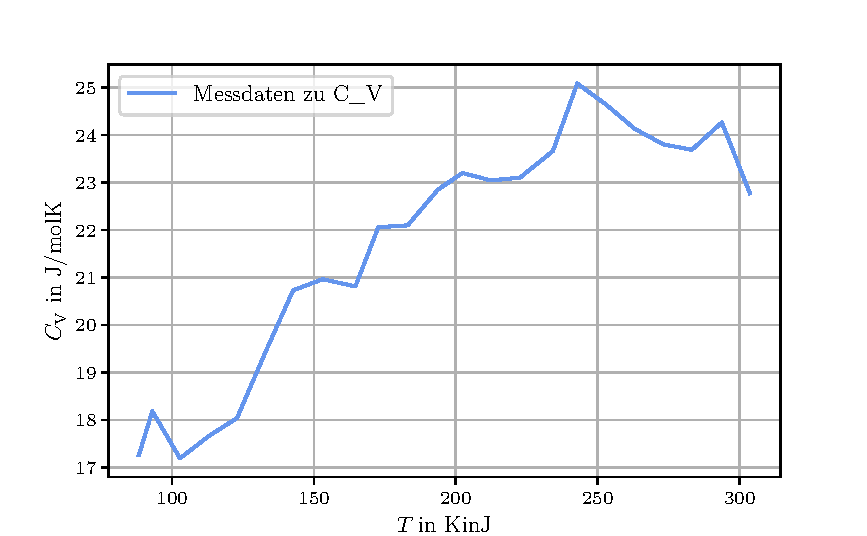
\includegraphics{build/c_v_plot.pdf}
    \caption{Specific heat capacity $C_\mathrm{V} dependet on the temperature$.}
    \label{fig:c_v}
\end{figure}
\begin{table}[htbp] 
    \centering 
    \begin{tabular}{cc c| ccc} 
        \toprule $T/\unit{\kelvin}$ & $\alpha/\unit{10^{-6}\frac{1}{\kelvin}}$ & $C_V / \unit{\frac{\joule}{\mol\kelvin}} $ & $T/\unit{\kelvin}$ & $\alpha/\unit{10^{-6}\frac{1}{\kelvin}}$ & $C_V / \unit{\frac{\joule}{\mol\kelvin}} $\\ 
        \midrule 
        84.59  & 9.074 & - & 193.69 &  14.8 &  22.85  \\   
        88.37  & 9.55  & 17.26 & 202.39 & 15.01 & 23.20    \\
        93.10  & 10.04 & 18.18  & 212.37 & 15.25 & 23.04     \\
        102.83 & 10.93 & 17.19  & 222.64 & 15.45 & 23.10    \\
        113.09 & 11.69 & 17.66  & 234.21 & 15.66 & 23.66     \\
        122.91 & 12.26 & 18.04 & 242.81 & 15.79 & 25.09    \\
        133.27 & 12.81 & 19.47  & 252.96 & 15.96 & 24.64     \\
        142.70 & 13.27 & 20.73  & 263.15 & 16.15 & 24.13    \\
        153.15 & 13.69 & 20.96  & 273.13 & 16.28 & 23.81 \\
        164.62 & 14.06 & 20.81 & 283.15 & 16.39 & 23.68     \\
        172.71 & 14.32 & 22.06  & 293.73 & 16.56 & 24.27    \\
        183.06 & 14.58 & 22.09 & 303.57 & 16.70 &  22.78   \\

        \bottomrule 
    \end{tabular} 
    \caption[Tabelle]{Calculated values for the linear thermal expansion coefficient and the specific heat capacity at constant volume.} 
    \label{tab:cv} 
\end{table}

\section{The Debye temperature of copper}

To determine the debye temperature $\theta_D$ of the sample, \autoref{fig:debye} is needed. It yields the value for $\frac{\theta_D}{T}$ for a certain $C_V$.
The result is then multiplied by the temperature the $C_V$ was calculated for. This gives the debye temperature $\theta_D$. The values can be seen in \autoref{tab:debye}.\\
The mean and error of the debye temperature is 
\begin{equation}
    \theta_D = 288.67 \pm 8.62 \, K.
\end{equation}
\begin{table}[htbp] 
    \centering 
    \begin{tabular}{cccc} 
        \toprule $T/\unit{\kelvin}$ & $C_V / \unit{\frac{\joule}{\mol\kelvin}} $ & $\frac{\theta_D}{T}$ & $\theta_D/\unit{\kelvin} $\\ 
        \midrule 
        84.59  & -      & - &     -     \\   
        88.37  & 17.26 &  2.8  &  247.43        \\
        93.10  & 18.18  &  2.6 &  242.06    \\
        102.83 & 17.19  &  2.8 &  287.93  \\
        113.09 & 17.66  & 2.7  &  305.34 \\
        122.91 & 18.04 &  2.6  &  319.57   \\
        133.27 & 19.47  & 2.3  &  306.51   \\
        142.70 & 20.73  & 2.0  &  285.39   \\
        153.15 & 20.96  &  1.9 &  290.98    \\
        164.62 & 20.81 &   1.9 &  312.78 \\
                
        \bottomrule 
    \end{tabular} 
    \caption[Tabelle]{Calculated values for the Debye temperature.} 
    \label{tab:debye} 
\end{table}

\begin{figure}
    \centering
    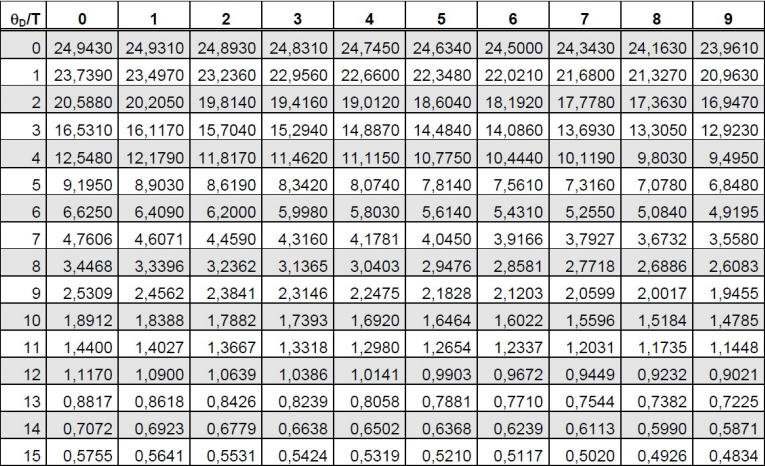
\includegraphics[scale=0.6]{content/V47_pictures/debyetemp.PNG}
    \caption{This is a table to calculate the debye temperature.}
    \label{fig:debye}
  \end{figure}

\section{Theoretical calculation of Debye-frequency and the Debye-temperature}
\label{sec:theo}
The theoretical value of the debye-frequency can be calculated using equation \ref{eqn:omega_D}. 
\begin{equation}
    \label{eqn:omega_D}
    \omega_\mathrm{D}^3 = \frac{18\pi^2N_\mathrm{A}}{V_0}\left(\frac{1}{v_{\mathrm{long}}^3}+\frac{2}{v_{\mathrm{trans}}^3}\right)^{-1}
\end{equation}
This equation derives from equation \ref{eqn:freq_dens}, by calculating the density state function $Z(\omega)$. In this equation $v_{\mathrm{long}}$ is the logitudinal phase velocity and
$v_{\mathrm{trans}}$ is the transversal phase velocity\cite{v47}. $N_\mathrm{A} = \qty{6.022e23}{\per\mol}$ is the \textit{Avogadro constant} and $V_0$ the molar volume of the sample.
The theoretical value of the debye-frequency is $\omega_\mathrm{D} = \qty{4.35e13}{\per\second}$. From this the debye-temperature can be calculated using equation \ref{eqn:theta_d}.
With the boltzmann constant this results in $\Theta_\mathrm{D} = \qty{332.18}{\kelvin}$

  